\documentclass[10pt, journal, letter, onecolumn]{IEEEtran}
\usepackage{amsmath,textcomp,amssymb,geometry,graphicx,verbatim}
\usepackage{fancyhdr}
\usepackage{caption}
\usepackage{subcaption,wrapfig,cite}
\usepackage{enumerate}


\usepackage{listings}
\usepackage{color}

\usepackage{indentfirst} % indent after section
\usepackage{mathtools}



\definecolor{dkgreen}{rgb}{0,0.6,0}
\definecolor{gray}{rgb}{0.5,0.5,0.5}
\definecolor{mauve}{rgb}{0.58,0,0.82}

\lstset{frame=tb,
  language=Java,
  aboveskip=3mm,
  belowskip=3mm,
  showstringspaces=false,
  columns=flexible,
  basicstyle={\small\ttfamily},
  numbers=none,
  numberstyle=\tiny\color{gray},
  keywordstyle=\color{blue},
  commentstyle=\color{dkgreen},
  stringstyle=\color{mauve},
  breaklines=true,
  breakatwhitespace=true,
  tabsize=4
}

\begin{document}
\title{Time Synchronization for High Performance Internet of Things Applications}

\author{
    Jessica Ko and Vasuki Narasimha Swamy
}
\maketitle
\bstctlcite{BIBcontrol}

The ``Tactile Internet'' promises to introduce several new emerging technology market opportunities like immersive and interactive applications such as robotics, gaming, smart-health-care, and smart grid.
To enable these high-performance IoT applications, ultra-reliable communication with latencies of about $1$ms is crucial.
This domain is largely unexplored and the techniques used by existing standards are fundamentally ill suited for low-latency and high-reliability.

An existing domain which parallels these requirements is high performance industrial control systems which are supported by wired communication protocol.
They support short messages (10s of bytes) to/from closeby sensors/actuators (10s -100s) delivered regularly (100s - 1000s of times per second). The protocols are ultra-reliable (probability of a single packet delivery failure of $10^{-8}$) with very low latency (a couple of ms).
Synchronized cooperative communication based wireless protocols proposed in \cite{swamy2015cooperative, swamy2016cooperative} achieves QoS (high-reliability and low latency) similar to wired fieldbus systems by exploiting multi-user diversity and distributed space-time coding to achieve.
One of the main requirements for protocols aiming at high-performance IoT applications is tightly synchronized clocks to avoid collision and thus avoiding any decoding errors which lead to violation of latency requirements.

To understand the kind of tight synchronization required we do the following back of the envelope calculations. Consider the ``Occupy CoW'' protocol described in \cite{swamy2015cooperative}. Each downlink and uplink messages are flooded into the network and all the nodes which can aid the origin node in getting the packet through to the destination help at the same time by the means of a distributed space time code (DSTC) - either a deterministic one like Alamouti \cite{alamouti1998simple}, or a random one like a random linear combination of possible codewords \cite{sirkeci2007randomized} or something even more simpler like delay diversity \cite{bossert2002cyclic}. The main objective of any DSTC is to enable full diversity. Thus each message gets two chances to reach the destination. If there are $25$ nodes in the network and the total time available is $2$ms, then the uplink packets get approximately $20 \mu$s. To ensure that uplink messages are decodable and everything happens in a timely fashion, the clocks need to be synchronized upto to a precision of $100$ns. The reason we can tolerate errors up to $100$ns is because an OFDM-like technique is employed can compensate for such offsets.

We studied some of the commonly used techniques for clock synchronization.
GPS clocks have great accuracy --- about $40 ns$. But there are two main reasons for why GPS clocks are not useful for our applications: (a) they work only outdoors (b) they have a very high convergence time.
The Internet generally synchronizes in a hierarchical fashion based on the seminal work of Mills ``Network Time Protocol''(NTP) \cite{mills1991internet}.
The offsets achieved by this protocol is in the order of hundreds of milliseconds and is clearly not good enough for us.
Reference broadcast based protocols \cite{elson2004global, elson2002fine} are a significant improvement over NTP as the offsets are in the order of microseconds and also deal well with skews (difference of clock frequencies).
Thus none of these already established methods were good enough for our application which requires accuracy in the order of $100 ns$. So we explored some simple methods inspired by these existing application. Section \ref{sec:clock} presents different clock models, section \ref{sec:setup} describes the problem in detail, section \ref{sec:methods} describes the methods explored for synchronization and \ref{sec:results} present the results.

\section{How do clocks work?}
\label{sec:clock}
In order to develop a synchronization protocol, we need to first understand the behavior of typical clocks. Clocks are made up of oscillators and a counter. Every time the oscillator finishes one oscillation it increments (or decrements) the counter. This is the smallest time that can be measured by the clock. For example if the oscillator was ticking at $10$ GHz, then the smallest time kept would be $\frac{1}{10 \times 10^{9}}$ which is $100$ps. More generally clocks tick at a frequency $F_c$ leading to a cycle time $T_c = \frac{1}{F_c}$. This is illustrated in Fig.~\ref{fig:clock_ideal}.

\begin{figure}[htb]
\begin{subfigure}[b]{0.45\textwidth}
\centering
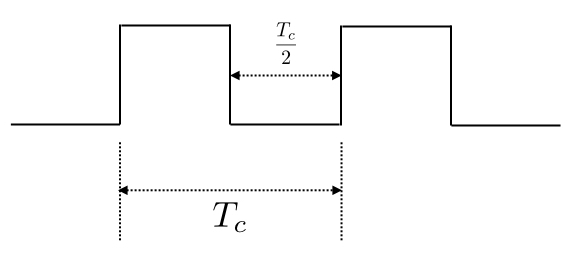
\includegraphics[width = \textwidth]{figures/ideal_clock}
\caption{Ideal clock}
\label{fig:clock_ideal}
\end{subfigure}
~\begin{subfigure}[b]{0.54\textwidth}
\centering
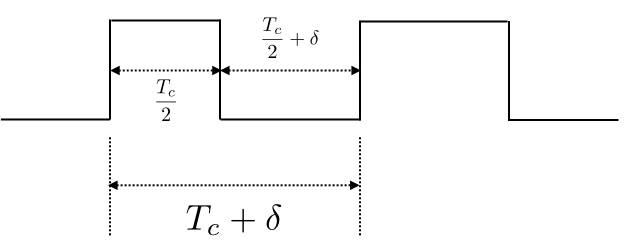
\includegraphics[width = \textwidth]{figures/real_clock}
\caption{Real clock}
\label{fig:clock_real}
\end{subfigure}
\caption{Ticking of different clocks}
\end{figure}

But these are ideal clocks. Most clocks are marked to tick at a frequency $F_c$ but they do not necessarily tick at that rate. The error in the actual ticking frequency of a `moderately good' clock is about $300$ ppm (parts per million). Thus if we are looking at a clock which is marked to tick at $10$GHz and if off by $300$ ppm, then it would be actually ticking at $10$ + $10 \times 300 \times 10^{-6}$ GHz which is $10.003$ GHz. While an ideal clock would report that $1$ second is $1$ second, the fast clock would report that the elapsed time is $1$ second and $30$ microseconds instead of $1$ second. The deviation from the ideal ticking rate is called the `skew' (denoted by $\alpha$) and this is the ratio between actual ticking rate and ideal ticking rate. Thus a clock $C(t)$ can be modeled as $C(t) = \alpha t + \beta$ where $t$ is the time at the ideal clock, $\alpha$ is the skew and $\beta$ is some initial offset.

What we described above is still a bit ideal. Why? We've completely ignored any environmental factors (like temperature, humidity, pressure) that might affect the oscillator's ticking rate \cite{frerking2012crystal}. These are important factors to be considered and actual oscillators behave differently. If the ideal frequency of oscillation is $F_c$ (leading to a period of $T_c$) then each period of oscillation in reality is $T_c + \delta$ where $\delta$ can be modeled as a Gaussian random variable \& this is called the jitter. This is illustrated in Fig.~\ref{fig:clock_real}. How high is the jitter going to be in one cycle? Typically, the standard deviation of $\delta$ is $50$ppm of $T_c$. In $1$ms, the number of cycles recorded by a $10$GHz oscillator ($T_c = 100$ps is $10 \times 10^{9} \times 10{-3} = 10^{7}$. Thus, if the standard deviation per cycle is $50$ppm of $100$ps, the standard deviation time taken to register $1$ms is $\left(\sqrt{10^7} \times 100 \times 50 \times 10^{-6}\right)$ps which is approximately $158$ps. This essentially means that the time needed to record $1$ms is a Gaussian random variable centered at $1$ms with a variance os $158$ps.

\section{Network Setup}
\label{sec:setup}

We consider a network with a central controller ($C$) that wishes to send and receive separate messages to and from each client in a set of $N$ client, denoted by the set $\mathcal{S}$ (see Fig.~\ref{fig:setup}). Distinct messages flow in a star topology from the central controller to individual clients, and in the reverse direction from the clients to the controller within a ``cycle'' of length $T$ (here $T = 2$ms). This cycle of communication must be achieved with a very small outage probability (on order of $10^{-9}$).

\begin{wrapfigure}{r}{0.3\textwidth}
  \begin{center}
    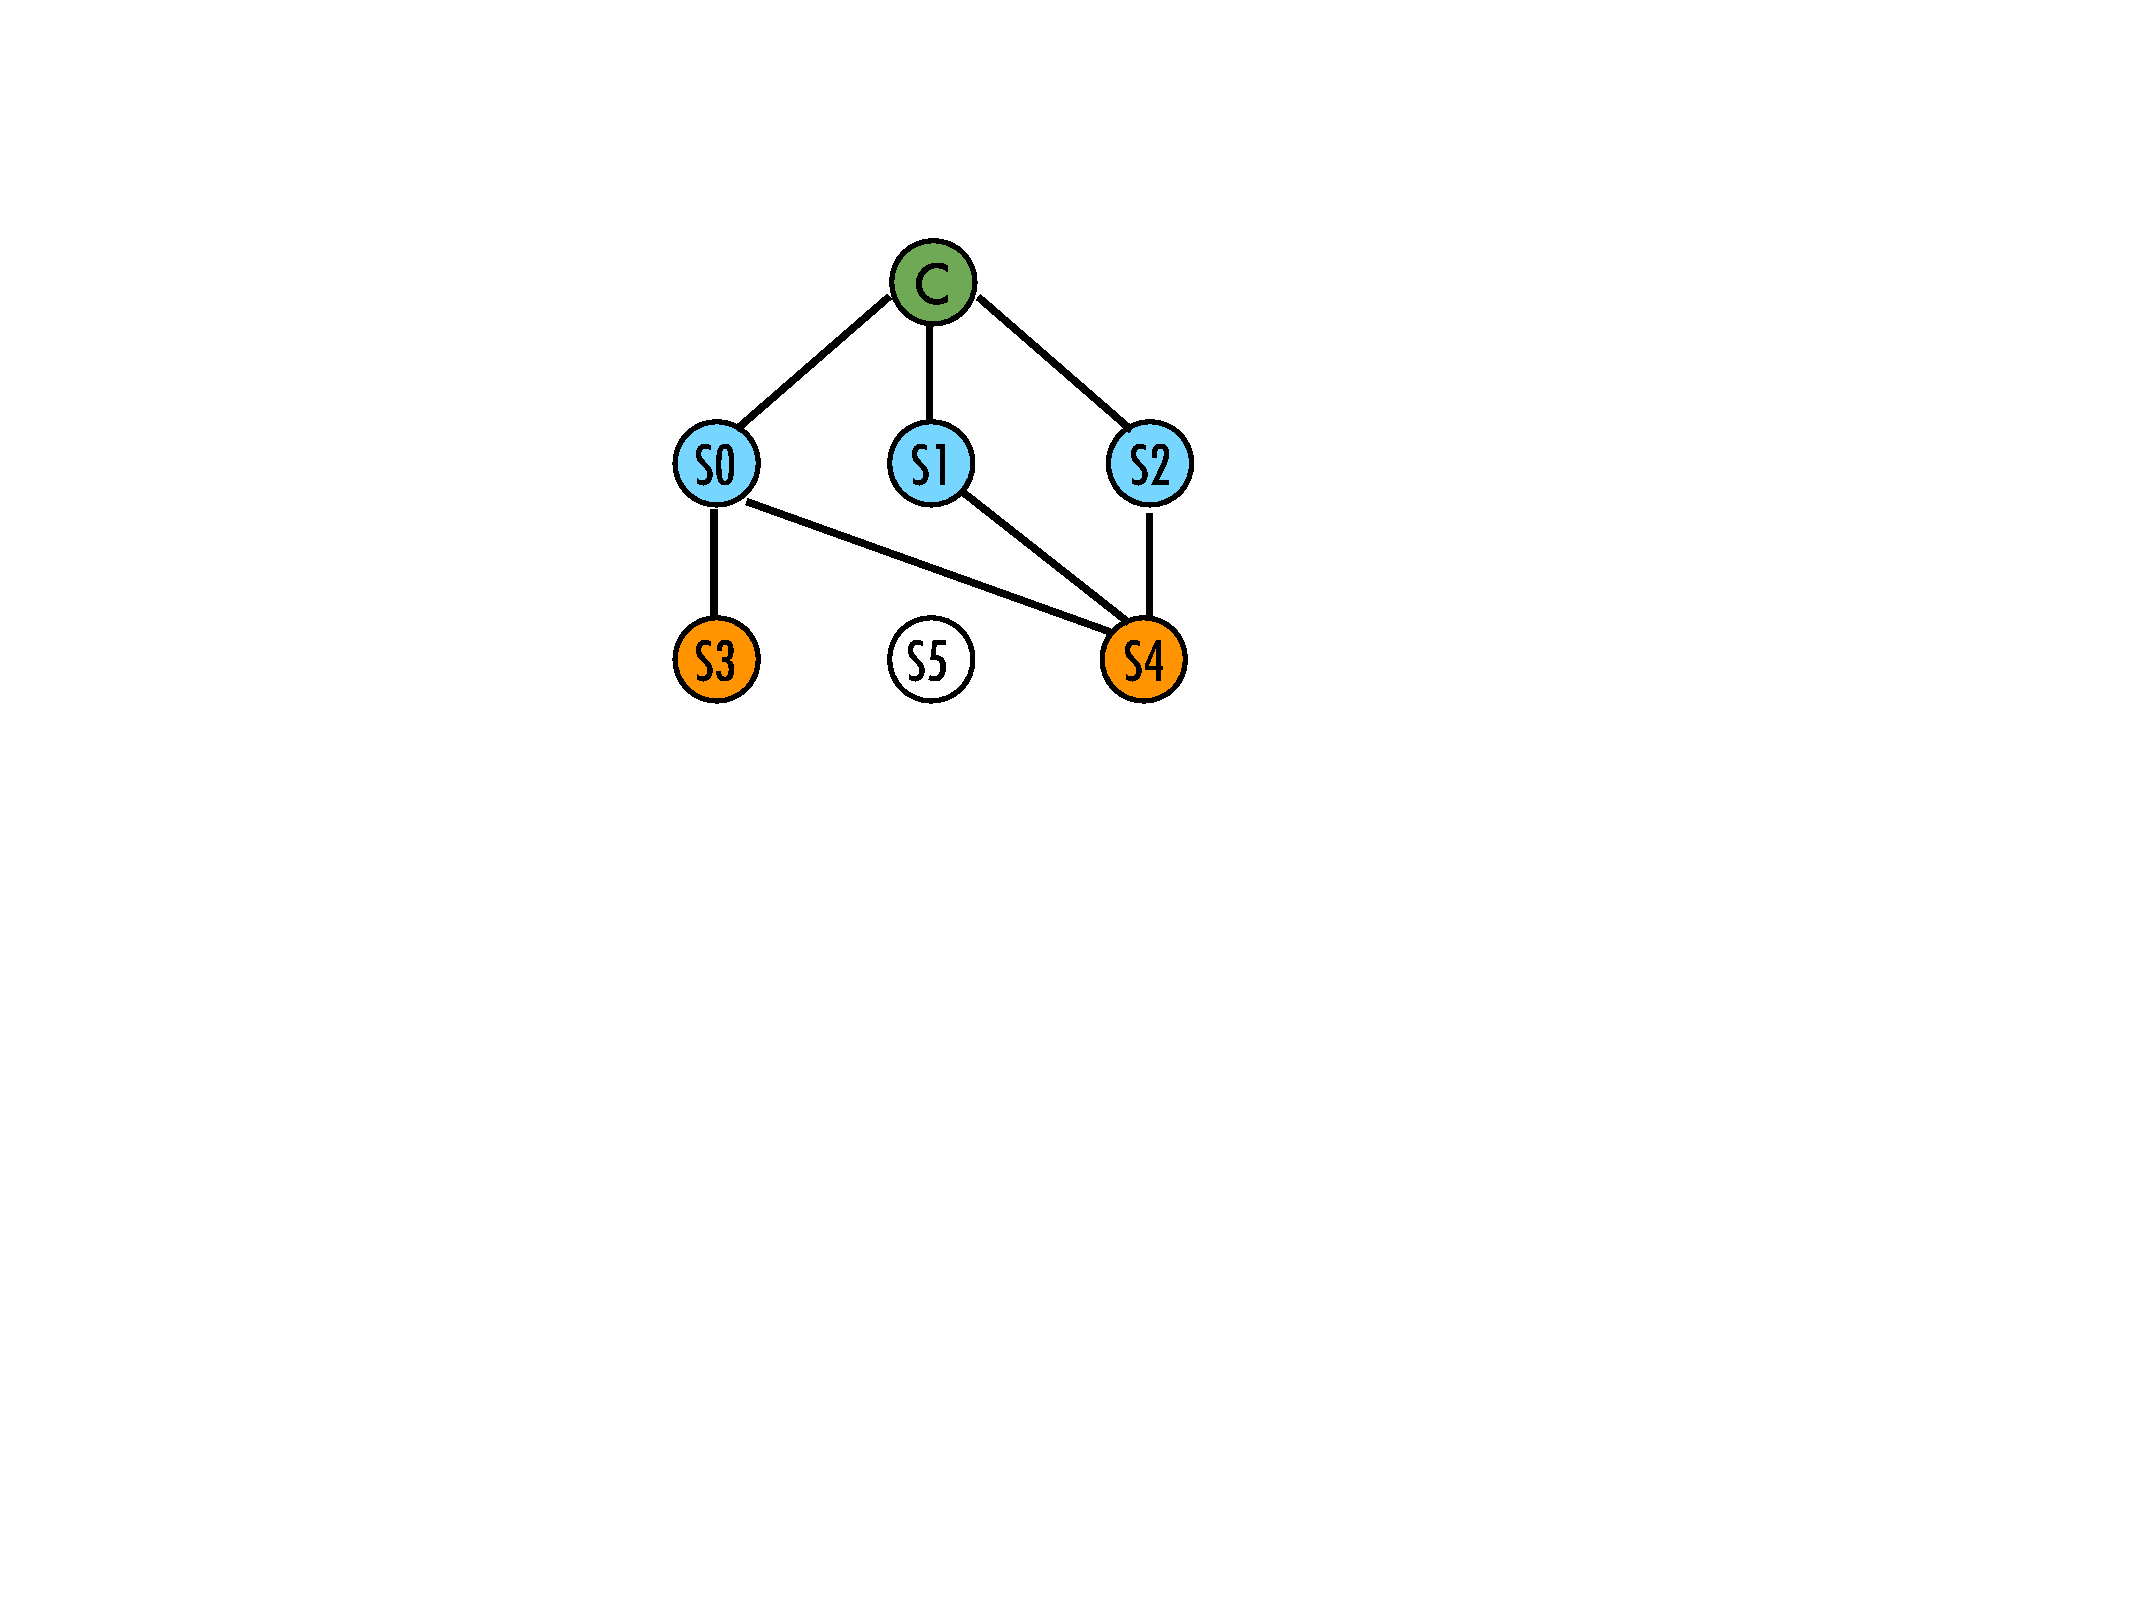
\includegraphics[scale = 0.5]{figures/bubbles_3}
  \end{center}
  \caption{Topology schematic for the protocols.}
  \label{fig:setup}
\end{wrapfigure}

The Occupy CoW protocol described in \cite{swamy2015cooperative} uses multi-user diversity to overcome bad fading events. The basic idea is to use a flooding strategy where the controller broadcasts a packet that includes messages for all clients. As this is a broadcast message, the intended set of recipients are all clients. Clients with good channels act as relays for other clients. This is done in a carefully scheduled, phased manner with dedicated time slots for each client to talk.

We first consider an aggressive synchronization protocol for the intial ideal clock model (where there is no jitter). As the applications we envision are mostly indoors (else we could just use GPS), most of the clients are in each other's range. We first consider a multiple beaconing reference clock model where there are several dedicated clock nodes say on the ceiling of each room which serve as reference clocks. These reference clocks are all connected by a wire so that they have the same reference time $t$.
The clocks in the $N$ clients are essentially marked to be ticking at the same rate as the reference clock but due to the imperfect nature of clocks, each client clock has a skew $\alpha_i$.
The time of client $i$ at time $t$ of the reference clock is $C_i(t) = \alpha_ i t + \beta_i$ where $\alpha_i$ is the skew and $\beta_i$ is the initial offset. Clients will listen to the messages of the closest reference clock. Figure \ref{fig:clock_model} shows the model with reference clocks and clients where $d_i(t)$ is the distance of client $i$ from the nearest reference clock at time $t$.

\begin{figure}[h]
    \centering
    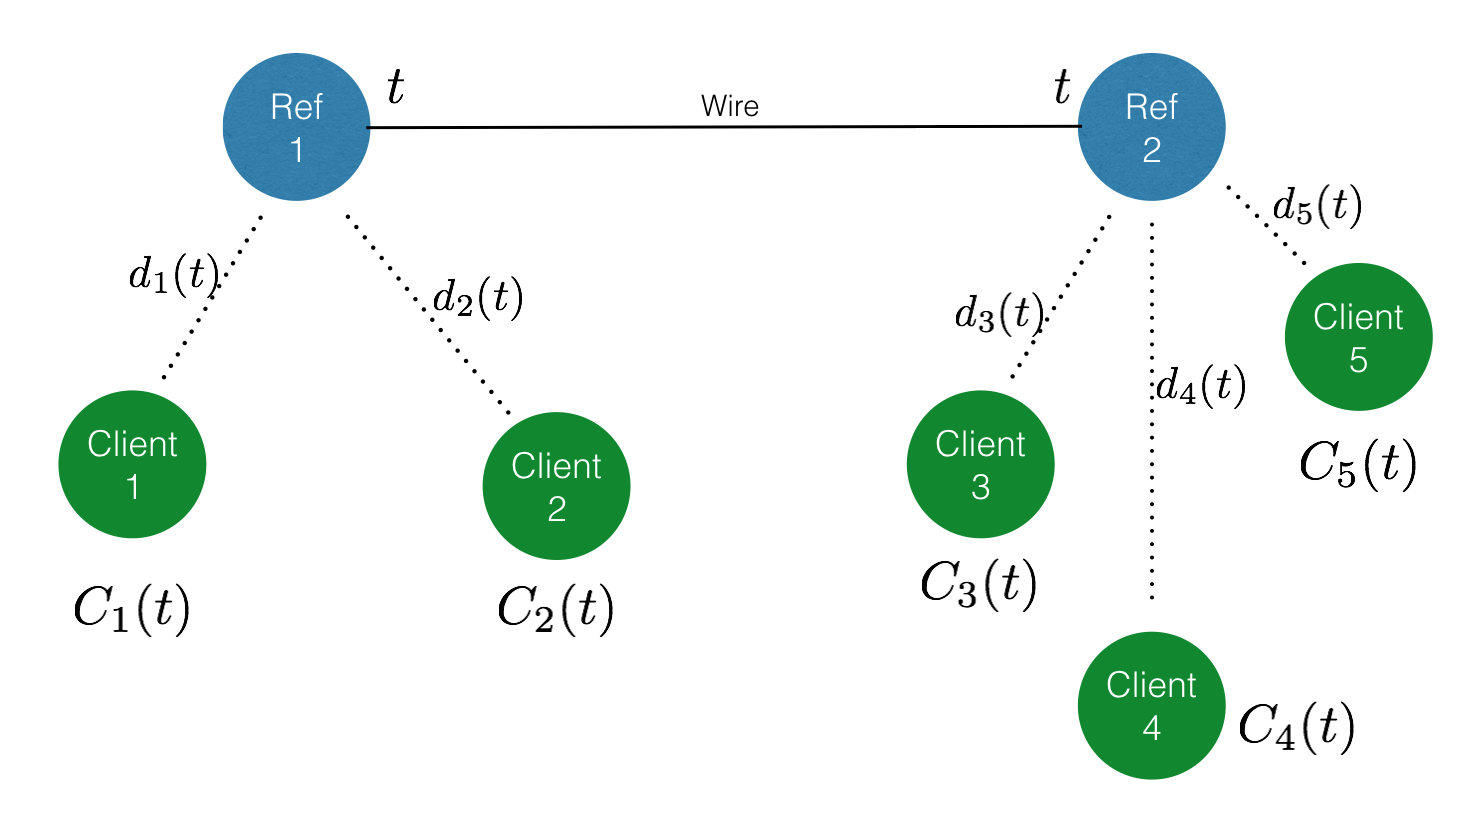
\includegraphics[scale=0.4]{figures/figure1}
    \caption{Clock Model}
    \label{fig:clock_model}
\end{figure}

The key feature of our synchronization protocol is that the reference clocks transmit a beacon indicating the time \emph{every} $t_0$ seconds. The clients are in promiscuous listening mode so they anticipate a beacon to arrive every $t_0$ seconds. The $t_0$ selected effects how fast the method converges to an accurate $\alpha$ and $\beta$ which we will discuss in detail in section \ref{sec:results}. After $k$ time intervals or at time $kt_0$, the reference clock will broadcast the time $kt_0$. The client $i$ will receive the message not exactly at $kt_0$ but after some time $n_i(k t_0)$ which is the combination of speed-of-light lag (which is inevitable) and recording lag (after all it takes time for the radio to figure out that it is receiving a packet). With a slight abuse of term we will call this `noise'.

\begin{figure}[htb]
    \centering
    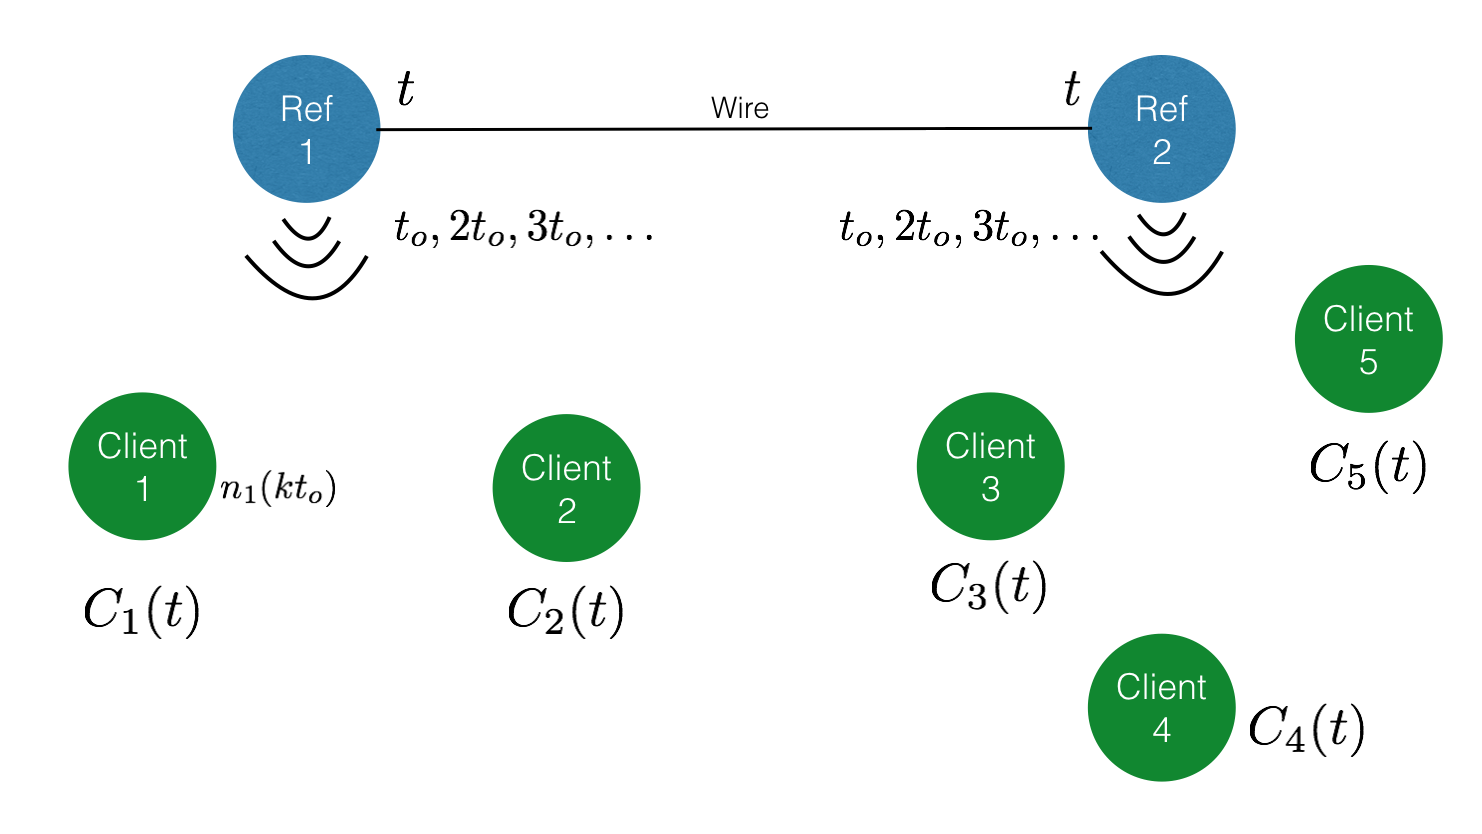
\includegraphics[scale=0.4]{figures/figure2}
    \caption{Clock Model  with Broadcasts and Noise}
    \label{fig:ref_broadcast}
\end{figure}

Noise is inevitable when the client receives the message from the reference clock. The noise for client $i$ is represented by $n_i(k t_0) \vcentcolon = n_i(k)$. The delay $d_i$ is determined by the speed of light constraints on the distance between the client and the closest reference clock.
In addition, there will be noise from the environment which is denoted by $N_i(k)$ and is chosen to be a normal distribution, $N_i(k) \sim \mathcal{N}(0, \sigma^2)$. Combining the two components, the noise is $n_i(k) = d_i + N_i(k) $. This also captures the minute movements that the clients have made in the interval of $t_0$. Figure \ref{fig:ref_broadcast} shows clock model with the noise and reference clock broadcasts.

\section{Synchronization Methods}
\label{sec:methods}
The client $i$ can estimate an $\alpha_i$ by using the times from consecutive intervals. When the reference clock broadcasts at fixed time intervals, the clients will recover their own time and the messages received contains $t_0$ to be used by the client for finding the skew. To simplify the notation, consider $C_i(k) = C^{(rec)}_i(kt_0)$, which is the time the client records that it received the synchronization message.
When there is no noise or $n_i(k) = 0$, the skew value can be obtained correctly from consecutive synchronization messages using the following equations.
\begin{eqnarray*}
\begin{aligned}
C_i(k+1) - C_i(k) &= \alpha_i (k+1) t_0 - \alpha_i (k) t_0\\
&= \alpha_i \times t_0
\end{aligned}
\end{eqnarray*}
Therefore we get,
$$\hat{\alpha_i} = \frac{C_i(k+1) - C_i(k)}{t_0} $$

However, noise is always present, so $\hat{\alpha_i} \neq \alpha_i$. A cleverer method to minimize the effect noise has on the skew is to consider the first synchronization packet arrival time (or an appropriate older packet) instead of the consecutive times. The reason we mentioned an appropriately older packet is because nodes are constantly moving and the $d_i$ would vary widely if we consider the \emph{very} first packet. So an older packet such that the movement is not too pronounced is good enough. The revised expression for the estimate of $\alpha$ is
\[
\hat{\alpha_i} = \frac{C_i(k) - C_i(1)}{(k - 1) t_0} = \frac{\alpha_i ( (k-1) t_0 + n_i(k) - n_i(1) ) }{(k - 1) t_0}
\]

The estimated skew can be used to find the estimate of $\beta$ along with speed of light lag (combined), denoted by $\hat{\beta}_c$. The reason we cannot distinguish between $\beta$ and the combined value $\beta_c$ as the rank of the matrix we are dealing with is $2$ and the number of variables is $3$ \cite{freris2010fundamentals, freris2007fundamental, giridhar2006distributed, freris2011fundamental}. With these estimated values, the client synchronizes it's time as described by the following equation.
\[
\text{virtual clock}_i = \frac{C_i(k) - \hat{\beta}_{c}}{\hat{\alpha}}.
\]

We also modeled the noise as an exponential random variable which would offset better for changing distance. We proved bounds for when the noise is exponential.

\subsection{Find $P(| \hat{\alpha} - \alpha_1 | \leq \epsilon)$}
First find $\hat{\alpha}$ an estimation of $\alpha_1$.
\[c_1 = \alpha_1 t + \beta \] \\
If there are no errors, then
\[ c_1(t_1 + j t_0) - c_1(t_1) = j \alpha_1 t_0 \]
\[
\hat{\alpha} = \alpha_1 = \frac{c_1(t_1 + j t_0) - c_1(t_1)}{j t_0}
\] \\
With noise st $n_k \sim exp(\lambda)$,
\[
 c_1(t_1 + j t_0 + n_{j+1}) - c_1(t_1 + n_1) = j \alpha_1 t_0 + \alpha_1 (n_{j+1} - n_1)
\] \\
Using the above method of dividing by $j t_0$.
\[
\hat{\alpha} = \frac{ j \alpha_1 t_0 + \alpha_1 (n_{j+1} - n_1)}{j t_0} = \alpha_1 +  \frac{  \alpha_1 (n_{j+1} - n_1)}{j t_0}
\]
Finding the probability,
\[
P(| \hat{\alpha} - \alpha_1 | \leq \epsilon) = P(\hat{\alpha} - \alpha_1  \leq \epsilon) - P(\hat{\alpha} - \alpha_1  \leq -\epsilon)
\]
$P(\hat{\alpha} - \alpha_1  \leq \epsilon) $ = ?
\[
P( \hat{\alpha} - \alpha_1  \leq \epsilon ) = P \left( n_{j+1} - n_1 \leq \frac{j t_0 \epsilon}{\alpha_1} \right)
\]
\begin{equation}
P \left( n_{j+1} - n_1 \leq \frac{j t_0 \epsilon}{\alpha_1} \right) = 1 - \frac{1}{2} e^{ -\lambda  \frac{j t_0 \epsilon}{\alpha_1} }
\label{eq:eq1}
\end{equation}
For $P(\hat{\alpha} - \alpha_1  \leq -\epsilon) $, we get
\begin{equation}
P(\hat{\alpha} - \alpha_1  \leq -\epsilon) = \frac{1}{2} e^{ -\lambda  \frac{j t_0 \epsilon}{\alpha_1} }
\label{eq:eq2}
\end{equation}
Putting Eq.~\eqref{eq:eq1} and \eqref{eq:eq2} together, we get
\begin{eqnarray}
\begin{aligned}
P(| \hat{\alpha} - \alpha_1 | \leq \epsilon)  &= 1 - \frac{1}{2} e^{ -\lambda  \frac{j t_0 \epsilon}{\alpha_1} } - \frac{1}{2} e^{ -\lambda  \frac{j t_0 \epsilon}{\alpha_1} }\\
&= 1 - e^{ -\lambda  \frac{j t_0 \epsilon}{\alpha_1} }
\label{eq:main}
\end{aligned}
\end{eqnarray}

\subsection{Find $E[ | \hat{\alpha} - \alpha_1 |^2 ]$}
Assume $\alpha_1$ to be a constant.
\begin{eqnarray}
\begin{aligned}
E[ | \hat{\alpha} - \alpha_1 |^2 ] &= E[\hat{\alpha}^2] - 2 E[\hat{\alpha} \alpha_1] + E[\alpha_1^2] = E[\hat{\alpha}^2] - 2 \alpha_1 E[\hat{\alpha}] + \alpha_1^2\\
&= E\left( \alpha_1 +  \frac{  \alpha_1 (n_{j+1} - n_1)}{j t_0}\right)^2 - 2 \alpha_1^2 + \alpha_1^2\\
&= \alpha_1^2 + \alpha_1^2 E\left[\left(\frac{(n_{j+1} - n_1)}{j t_0}\right)^2\right] - 2\alpha_1^2 E\left[\frac{(n_{j+1} - n_1)}{j t_0}\right]  - \alpha_1^2\\
&= \alpha_1^2 \left(E\left[\left(\frac{n_{j+1}}{j t_0}\right)^2\right] + E\left[\left(\frac{n_{1}}{j t_0}\right)^2\right] - 2 E\left[\frac{n_{j+1}}{j t_0}\right] E\left[\frac{n_{1}}{j t_0}\right] - 2E\left[\frac{n_{j+1}}{j t_0}\right] + 2E\left[\frac{n_{1}}{j t_0}\right]\right)\\
&= \alpha_1^2 \left( \frac{2}{\lambda^2} + \frac{2}{\lambda^2} - 2\frac{1}{\lambda}\frac{1}{\lambda}\right) + \alpha_1^2\left( \frac{2}{\lambda} - \frac{2}{\lambda} \right)\\
&= \frac{2\alpha_1^2}{\lambda^2}
\end{aligned}
\end{eqnarray}

These seem well enough for the ideal clock model with constant skew but what about the case when the clocks take a random walk along the line of constant skew? Does this method give us good enough results or do we have to do something more intelligent? Before answering that question, we explored how the above method would perform for ideal clocks.

\section{Results}
\label{sec:results}
We performed some initial simulations with one reference clock and four clients. Synchronization starts at the $60$th time interval, so the times of the client clocks before that time are not very accurate.

\begin{figure}[h]
\begin{subfigure}[b]{0.45\textwidth}
\centering
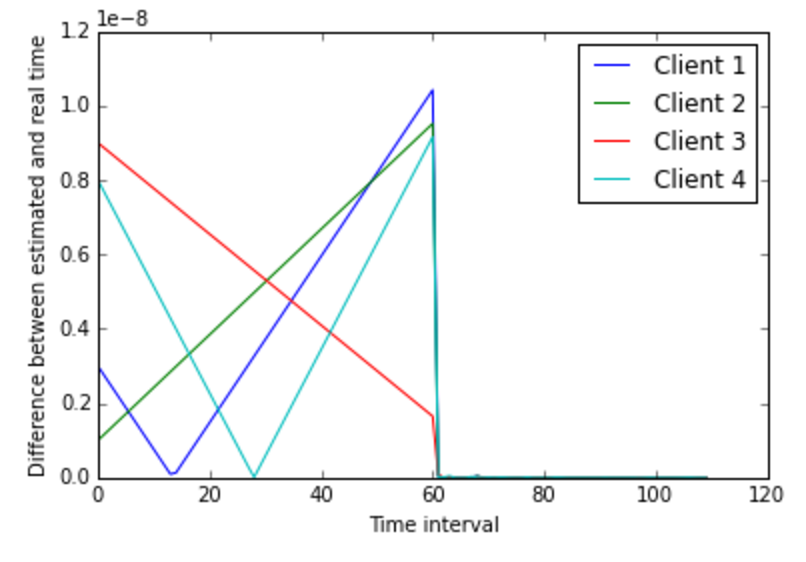
\includegraphics[scale=0.5]{figures/figure3}
\caption{Results when $t_0 = 1$ms}
\label{fig:results1_1ms}
\end{subfigure}~
\begin{subfigure}[b]{0.45\textwidth}
\centering
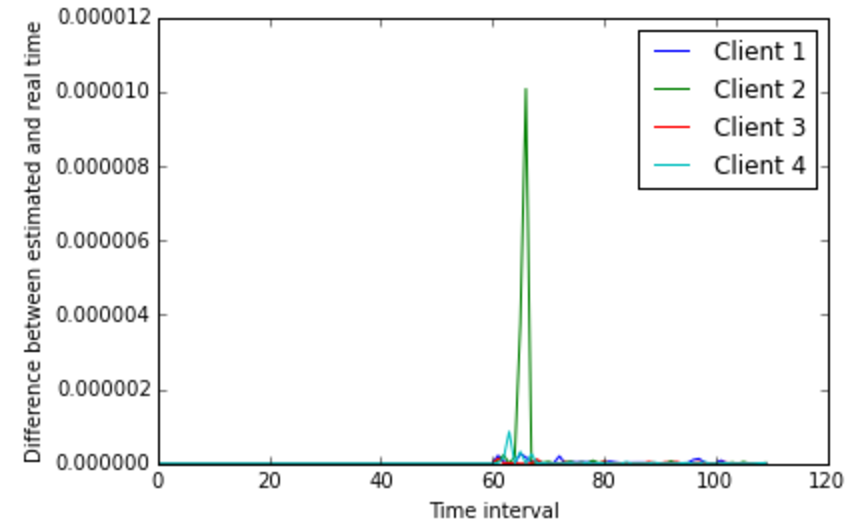
\includegraphics[scale=0.5]{figures/figure4}
\caption{Results when  $t_0 = 1 \mu s$}
\label{fig:results1_1mus}
\end{subfigure}
\label{fig:results1}
\end{figure}

For the clients, the skew is between $-300$ to $300$ ppm, which is an accurate representation of most clocks. The offset is picked randomly and the distance from the reference clock is picked randomly between $2$ to $10$ meters (this is fine as the applications being targeted are indoors and mostly in the line-of-sight of each other).
The standard deviation of the noise that we used in our simulations was $100$ns. This is a good estimate of any movement or wrong estimate from mean position + radio delay. The distance covered by a radio signal in $100$ns is $30$m and any moving radio would typically cover than distance in $10$ seconds or so. Given we are considering applications in indoor environment, it is safe to assume that at most $1$ns (or $30$cm) error is contributed due to inaccuracy in distance measurement in every cycle lasting about $1$ms. In addition to that, $100$ns noise also takes into account any delay in measurement and decoding. If we had a $10$Ghz oscillator then $100$ns corresponds to almost $1000$ symbols of error which is roughly the maximum delay in a radio circuit to declare that a packet is being transmitted.

When $t_0 = 1$ms as shown in Figure \ref{fig:results1_1ms}, the method performs extremely well because the difference between the estimate time and real time gets very close to zero within the first few time intervals.

From Eq~\eqref{eq:main} it is plenty clear that considering the length of the time interval is necessary because the results are influenced by what value is picked. When a shorter time interval is used, the accuracy of the estimated time is worse as shown in Figure \ref{fig:results1_1mus} with $t_0 = 1 \mu s$. This is supported by Eq.~\eqref{eq:main} which states that the probability that we get too far from the true value of skew is an increasing function of $t_0$ so the simulation results agree with the theory.
If a longer time interval like $10$ms is used, the accuracy of the estimated time improves. When looking at time intervals greater than 70, figures \label{fig:results2_1ms} and \label{fig:results2_10ms} easily show the difference between accuracies. However, an accurate estimated time takes longer to reach because the time intervals are now longer.

\begin{figure}
\begin{subfigure}[b]{0.45\textwidth}
\centering
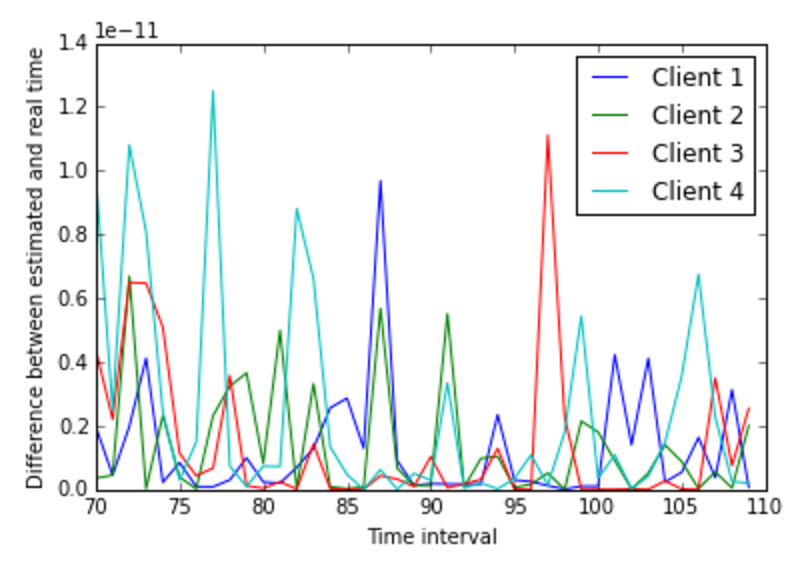
\includegraphics[scale=0.5]{figures/figure5}
\caption{Results when $t_0 = 1$ms for time past 70ms}
\label{fig:results2_1ms}
\end{subfigure}~
\begin{subfigure}[b]{0.45\textwidth}
\centering
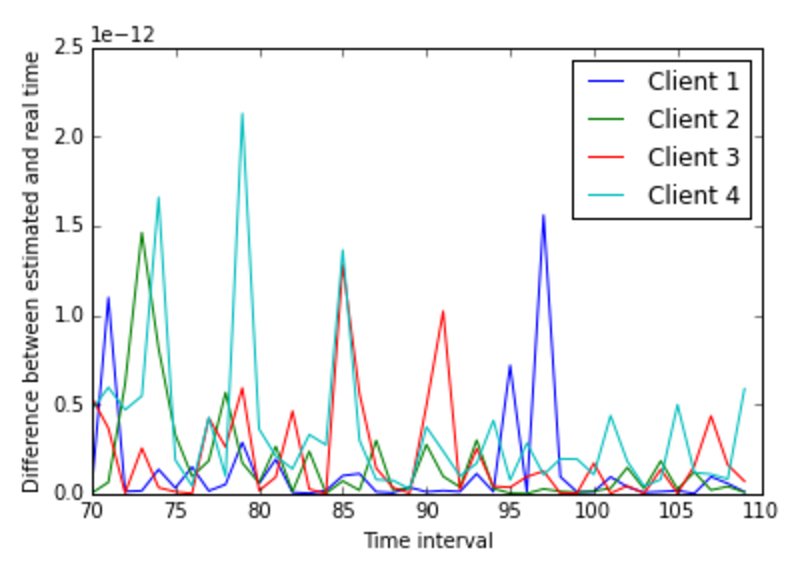
\includegraphics[scale=0.5]{figures/figure6}
\caption{Results when $t_0 = 10$ms for time past 70ms}
\label{fig:results2_10ms}
\end{subfigure}
\label{fig:results2}
\end{figure}

\bibliographystyle{IEEEtran}

\bibliography{IEEEabrv,cs268}


\end{document}